% !TeX root = ../thesis.tex

\chapter{Introduction}
\label{sec:introduction}

%\gls{ma} \gls{online_reference}

There are different kinds of object detection networks in the field of autonomous driving, some based on camera and some based on LiDAR. Research on the robustness of image object detection networks has been sufficient, but LiDAR-based as a new sensor based object detection networks have achieved considerable progress in the detection accuracy of different types of objects after several years of development. It can be seen from Figure 1.1 that different types of objects have relatively high detection accuracy. 
\begin{figure}[!htbp]
\centering
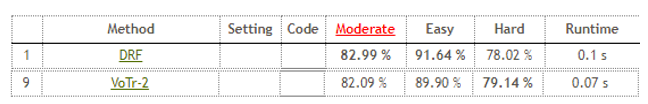
\includegraphics[scale=0.5]{Graphics/KITTI Leaderboards.png}
\caption{Current Best Results of Car Class on KITTI\cite{geiger_vision_2013} Learderboards}
\label{fig:KITTI Learderboards}
\end{figure}


\section{Motivation}
the robustness of LiDAR-based object detection model is still unknown. There may be two aspects that affect the robustness: one is adversarial attack, the other is adverse weather. Point clouds under adverse weather is point clouds, which LiDAR acquired under adverse weather, including rain, snow, fog, etc. From Figure 1.2 we could seen in the point clouds under adverse weather are significant different with clean point clouds. 
\begin{figure}[!htbp]
    \centering
    \subfigure[Clean Point Cloud\cite{geiger_vision_2013}]{
        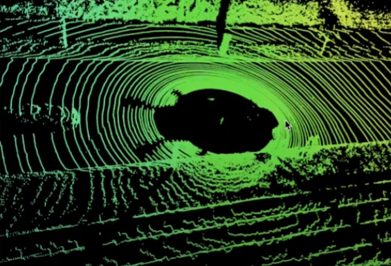
\includegraphics[width = \textwidth / 2 ]{Graphics/Clean Point Cloud.png}
        \label{fig:Clean Point Cloud}
    }
    \hspace{10pt}
     %add desired spacing between images, e. g. ~, \quad, \qquad, \hfill etc.
     %(or a blank line to force the subfigure onto a new line)
    \subfigure[Snow Point Cloud\cite{pitropov_canadian_2021}]{
        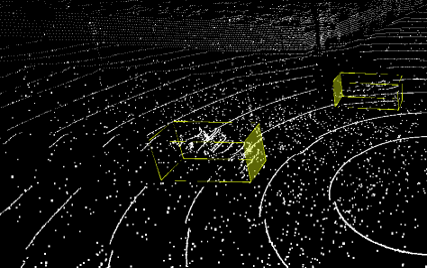
\includegraphics[width = \textwidth / 2 ]{Graphics/Snow Point Cloud.png}
        \label{fig:Snow Point Cloud}
    }
    \caption[Short Description for List of Figures]{The Differences between Clean Point Cloud and Snow Point Cloud}
    \label{fig:logo1and2}
\end{figure}
Most of the detection networks trained based on the clean point clouds may not be capable of the point clouds under adverse weather. Adversarial attack was first proposed in the field of image classification. The slight perturbation calculated with gradient is added to the original image to generate a perturbed image that is imperceptible to the naked eye, but will fool the classifier.
For point clouds detection model there's also gradient could be calculated from the loss, which could use the same method to fool the detection model.

\section{Goal Description}
For adversarial attack, slight changes to point clouds can also cause a substantial negative impact on 
the performance of detection model. For point clouds under adverse weather simulation, according to the character of point clouds under adverse weather, through adding, perturbing and dropping points methods to simulate the point clouds under adverse weather. In order for training a robust model when lack of adverse weather point clouds.
\paragraph{Contribution}
For adversarial attack there are three sections: 

the first section is FGSM. Many previous work have shown FGSM is efficient in image domain and point cloud classification domain\cite{liu_extending_2019}, this work have proved FGSM can also be applied in point cloud detection model. 

The second section is critical point drop attack. From some related studies, PointNet\cite{qi_pointnet_2017-1} defines critical points. PointPillars use a simplified PointNet to get critical features. Zheng et.al \cite{zheng_pointcloud_2019} proposed an adversarial attack by dropping critical points. By combining these thoughts, critical points in PointPillars could be defined as "critical" features in PointPillars, and execute an attack by dropping critical points. 

The first two sections are enforced on detection models.
In section three, we propose an adversarial attack method "points perturbation and points drop", it's not rely on detection model, so it can be applied in more networks. Using these methods, create benchmark datasets to test the robustness of more models. 

In the last section, simulate adverse weather point clouds to improve robustness by using additional data in adverse weather.


\section{Outline}
Introduction

Fundamentals and Related Work

Underlying Conditions and Preliminaries

Concepts

Implementations

Evaluation

Conclusion and Future work


